\section{Auswertung}
\label{sec:Auswertung}

\subsection{Ablenkung im elektrischen Feld}
Die Messdaten zur Untersuchung der Ablenkung von bewegten Elektronen im elektrischen Feld sind
in Tabelle \ref{tab:efeldtab} zu finden.
\begin{figure}
  \centering
  \includegraphics{Messdaten/plotefeld.pdf}
  \caption{Ablenkung $D$ am Leuchtschirm aufgetragen gegen die gemessene Ablenkspannungen $U_\mathrm{d}$ zur Bestimmung der Empfindlichkeit $\kappa_i$.}
  \label{fig:efeld}
\end{figure}

Zur Bestimmung der Empfindlichkeit $\kappa=\frac{D}{U_\mathrm{d}}$ der Kathodenstrahlröhre wird die Position $D$ des Auftreffspunkt am Leuchtschirm gegen die gemessene Ablenkspannung $U_\mathrm{d}$ für die gemessenen Beschleunigungsspannungen $U_\mathrm{B}$ in Abbildung \ref{fig:efeld} aufgetragen.
Hierbei wurde eine lineare Ausgleichsrechnung mittels scipy/python \cite{scipy} nach
\begin{equation*}
	y=m\cdot x+b
\end{equation*}
durchgeführt.
Aus dem Geradenparameter %huiii richtig geschrieben :P
$m$ ergibt sich schließlich die Empfindlichkeit $\kappa$ der Elektronestrahlröhre.
Für die verschiedenen Beschleunigungsspannungen $U_\mathrm{B}$ ergibt sich:
\begin{gather*}
	\kappa_{400\,\si{\volt}} =  \SI{0.117(5)}{\centi\meter\per\volt} \text{,}\\
	\kappa_{300\,\si{\volt}}  =  \SI{0.159(5)}{\centi\meter\per\volt} \text{,}\\
	\kappa_{200\,\si{\volt}}  =  \SI{0.250(6)}{\centi\meter\per\volt} \text{.}
\end{gather*}
\begin{figure}
  \centering
  \includegraphics{Messdaten/plotm.pdf}
  \caption{Empfindlichkeit $\kappa_i$ aufgetragen gegen die reziproke Beschleunigungsspannung $U_\mathrm{B}$.}
  \label{fig:m}
\end{figure}
In Abbildung \ref{fig:m} sind die bestimmten $\kappa_\mathrm{i}$ gegen die zugehörigen reziproken Beschleunigungsspannungen $U_\mathrm{B}$ aufgetragen.
Erneut wird mittels scipy/python \cite{scipy} eine lineare Ausgleichsrechnung durchgeführt.
Die Steigung $m$ der Ausgleichsgraden entspricht der Apparaturkonstanten $K$.
Mit Gleichung \eqref{eqn:K} ergibt sich
\begin{equation*}
	K= D \cdot \frac{U_\mathrm{B}}{U_\mathrm{d}}=\frac{p\cdot L}{2d} \text{.}
\end{equation*}
Die experimentell bestimmte Apparaturkonstante $K$ ist
\begin{equation*}
	K=m_\mathrm{Ausgleich} =  \SI{53(1)}{\centi\meter} \text{.}
\end{equation*}
Wird die Apparaturkonstante über die Abmessungen der Kathodenstrahlröhre ermittelt, ergibt sich mit $L=\SI{14.3}{\centi\meter}$, $p=\SI{1.9}{\centi\meter}$ und $d=\SI{0.38}{\centi\meter}$:
\begin{equation*}
	K=\SI{35.75}{\centi\meter}\text{.}
\end{equation*}

\begin{table}
	\caption{Messdaten zur Bestimmung der Empfindlichkeit $\kappa$ der Kathodenstrahlröhre.}
	\label{tab:efeldtab}
	\centering
	\begin{tabular}{cccc}
	\toprule
		& & $U_{\mathrm{d}}$ für & \\
		\midrule
		$D$ / \si{\centi\meter} & $U_{\mathrm{B}}=\SI{400}{\volt}$ & $U_{\mathrm{B}}=\SI{300}{\volt}$ & $U_{\mathrm{B}}=\SI{400}{\volt}$ \\
		\midrule
		0.000 & -7.70 & -8.2 & -6.0 \\
		0.635 & -5.40 & -5.4 & -4.3 \\
		1.270 & -1.72 & -1.5 & -1.6 \\
		1.905 & 5.62 & 3.1 & 0.9 \\
		2.540 & 9.00 & 5.4 & 3.1 \\
		3.175 & 14.95 & 9.5 & 5.4 \\
		3.810 & 22.60 & 14.2 & 8.4 \\
		4.445 & 28.40 & 19.1 & 11.5 \\
		5.080 & 33.00 & 23.5 & 14.0 \\
	\bottomrule
	\end{tabular}
\end{table}


\subsection{Untersuchung einer Sinusspannung mittels des Kathodenstrahl-Oszillographs}
In Tabelle \ref{tab:saegen} sind die gemessenen Frequenzen der Sägespannung eingetragen, bei denen eine Entartung des Oszilloskopbilds zu einer stehenden Welle festgestellt wurde. Zudem sind die zugehörigen Frequenzverhätnisse zwischen angelegter Wechselspannung und der Sägespannungsfrequenz $\nu_\mathrm{Säge}$ eingetragen.
\begin{table}
	\caption{Bestimmte Synchronisationsfrequenzen zur Erzeugung von stehenden Wellen auf dem Leuchtschirm.}
	\label{tab:saegen}
	\centering
	\begin{tabular}{cc}
	\toprule
		Frequenzverhältnis $n$ & $\nu_\mathrm{Säge}$ / $\si{\hertz}$ \\
	\midrule
		0.5 & 39.96 \\
		1.0 & 79.95 \\
		2.0 & 159.85 \\
		3.0 & 239.73 \\
	\bottomrule
	\end{tabular}
\end{table}
Eine Mittellung über alle Werte ergibt mittels python/numpy \cite{numpy} für die Frequenz der angelegten Sinusspannung:
\begin{equation*}
	\nu_\mathrm{Sinus}=\SI{79.926(9)}{\hertz} \text{.}
\end{equation*}



%\begin{figure}
%  \centering
%  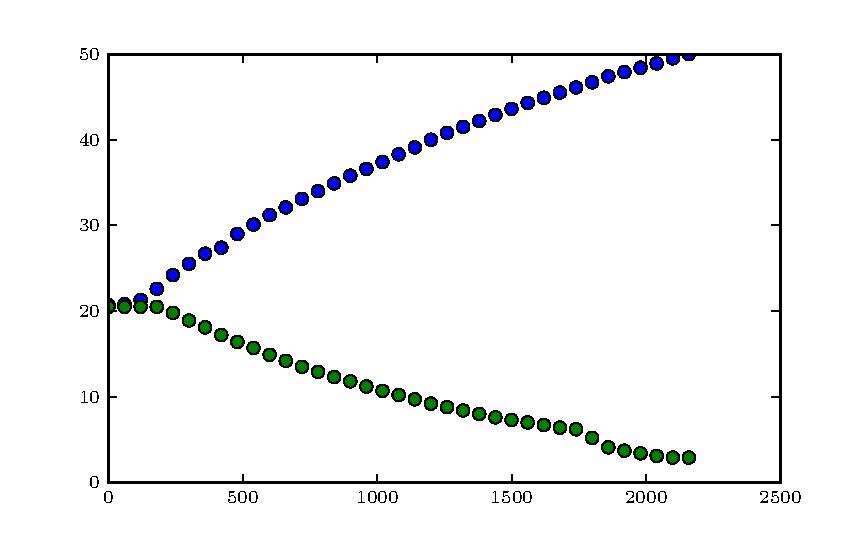
\includegraphics{plot.pdf}
%  \caption{Plot.}
%  \label{fig:plot}
%\end{figure}

%%%%%%%%%%%%%%%%%%%%%%%%%%%%%%%%%%%%%%%%%%%%%%%%%%%%%%%%%%%%%%%%%%%%%%%%%%%%%%%%%%%%%%%%%%%
\FloatBarrier
\subsection{Ablenkung im magnetischen Feld}

\subsubsection{Bestimmung von $\frac{\symup{e}_0}{\symup{m}_0}$}
Die Messergebnisse zur Berechnung von $\frac{\symup{e}_0}{\symup{m}_0}$ sind in Tabelle
\ref{tab:efeldtab} aufgetragen. Es wird eine lineare Ausgleichsrechnung der Form
\begin{equation*}
	y = m \cdot x + b
\end{equation*}
gemäß Formel \eqref{eqn:bfeld1} mit scipy/python \cite{scipy} durchgeführt. Hierbei entspricht das
$y$ dem Faktor $\frac{D}{L^2+D^2}$ und das $x$ der Flussdichte $B$.
Die Parameter für die Beschleunigungsspannung $U_{\mathrm{b}}=\SI{250}{\volt}$ ergeben sich zu
\begin{gather*}
	m = -\SI{15548(3386)}{\kelvin} \mathrm{,} \\
	b = \SI{2.6(3)}{\per\meter} \mathrm{.}
\end{gather*}
\begin{figure}
  \centering
  \includegraphics{Messdaten/plotbfeld.pdf}
  \caption{Ausgleichsgerade mit Messwerten für eine Beschleunigungsspannung von $U_{\mathrm{b}}=\SI{250}{\volt}$.}
  \label{fig:bfeldplot}
\end{figure}
Die Ausgleichsgerade mit den Messwerten ist in Abbildung \ref{fig:bfeldplot} dargestellt.
Analog lassen sich die Parameter für die Beschleunigungsspannung $U_{\mathrm{b}}=\SI{450}{\volt}$
zu
\begin{gather*}
	m = -\SI{13662(2964)}{\kelvin} \mathrm{,} \\
	b = \SI{2.8(4)}{\per\meter}
\end{gather*}
\begin{figure}
  \centering
  \includegraphics{Messdaten/plotbfeld2.pdf}
  \caption{Ausgleichsgerade mit Messwerten für eine Beschleunigungsspannung von $U_{\mathrm{b}}=\SI{450}{\volt}$.}
  \label{fig:bfeldplot2}
\end{figure}
bestimmen. Die Ausgleichsgerade ist in Abbildung \ref{fig:bfeldplot2} dargestellt.
\begin{table}
	\caption{Messwerte für die Verschiebung $D$ in Abhängigkeit vom Spulenstrom bei Beschleunigungsspannungen von $U_{\mathrm{b}}=\SI{250}{\volt}$ und $U_{\mathrm{b}}=\SI{450}{\volt}$.}
	\label{tab:bfeldtab}
	\centering
	\begin{tabular}{ccc}
	\toprule
		$D$ / $\si{\centi\meter}$ & $I$ / $\si{\ampere}$ bei $U_{\mathrm{b}}=\SI{250}{\volt}$ & $I$ / $\si{\ampere}$ bei $U_{\mathrm{b}}=\SI{450}{\volt}$ \\
	\midrule
		0.635 & 0.35 & 0.46 \\
		1.270 & 0.67 & 0.83 \\
		1.905 & 0.98 & 1.26 \\
		2.540 & 1.21 & 1.69 \\
		3.175 & 1.57 & 2.09 \\
		3.810 & 1.90 & 2.52 \\
		4.445 & 2.21 & 2.94 \\
		5.080 & 2.53 & - \\
	\bottomrule
	\end{tabular}
\end{table}
Damit ergeben sich die Verhältnisse gemäß Formel \eqref{eqn:bfeld1} und scipy \cite{scipy} zu
\begin{gather*}
	\frac{\symup{e}_0}{\symup{m}_0}_{\mathrm{theo}} =  -\SI{175.8820024(24)}{\giga\coulomb\per\kilo\gram} \mathrm{,} \\
	\frac{\symup{e}_0}{\symup{m}_0}_{U_{\mathrm{b}} = \SI{250}{\volt}} = -\SI{480(210)}{\giga\coulomb\per\kilo\gram} \mathrm{,} \\
	\frac{\symup{e}_0}{\symup{m}_0}_{U_{\mathrm{b}} = \SI{450}{\volt}} = -\SI{900(400)}{\giga\coulomb\per\kilo\gram} \mathrm{,}
\end{gather*}
mit der Elementarladung nach \cite{e} und der Elektronenmasse nach \cite{m} für den Theoriewert.
\subsection{Bestimmung der Intensität des lokalen Erdmagnetfelds}
Zur Bestimmung der Intensität des lokalen Erdmagnetfelds wird zunächst mittels des Deklinatorium-Inklinatoriums der lokale Inklinationswinkel des Erdmagnetfelds zur Horizontalebene zu $\alpha=75^\circ$.
Nach Formel \eqref{eqn:b-feld} wird die Flussdichte $B$ des Ausgleichsfeld bestimmt.
Hierbei beträgt der Spulenstrom $I=\SI{0.25}{\ampere}$, die Windungszahl der Helmholtzspule $N=20$ und der Spulenradius $R=\SI{0.282}{\meter}$.
Es ergibt sich:
\begin{equation}
  B_\mathrm{Ausgleich}=\SI{1.59e-05}{\tesla} \text{.}
\end{equation}
Zur Bestimmung der Intensität des lokalen Erdmagnetfelds muss der berechnete Wert noch durch den Kosinus des Inklinationswinkel dividiert wird.
Diese ergibt sich schließlich zu:
\begin{equation}
  B_\mathrm{Erde}=\SI{6.16e-05}{\tesla} \text{.}
\end{equation}
